\chapter{Auxiliary definitions}

\section{Graphs}

\paragraph{}
A graph is a mathematical structure, describing the relations between a set of objects. The objects are represented as vertices (or nodes) in the graph while the relations are represented as the edges between those vertices. Usually, a graph is depicted using a set of dots or circles for vertices joined by straight lines for edges as indicated in \autoref{fig:simple_graph}. 

\paragraph{}
A graph (G) could be represented as \(G = (V, E)\) where, \(V\) is the set of vertices and \(E \in \{\{x, y\} | (x, y) \in V^2 \wedge x \ne y\}\) is the set of edges

\begin{figure}[H]
    \centering 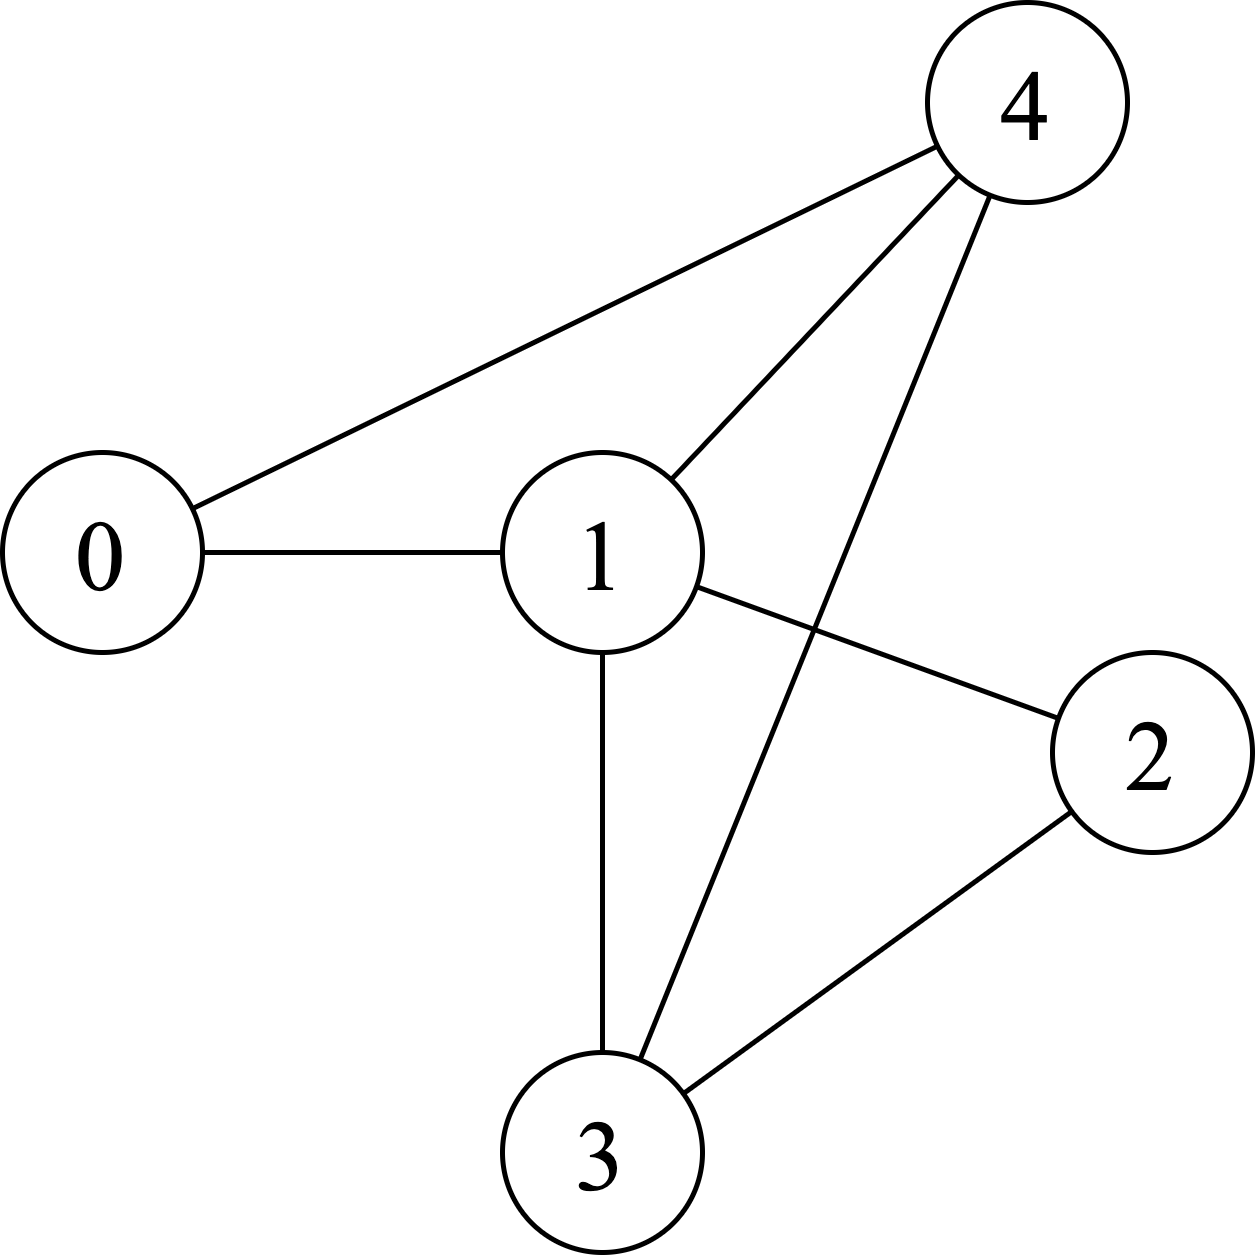
\includegraphics[width=0.4\textwidth]{simple_graph}
    \caption{A simple graph}
    \label{fig:simple_graph}
\end{figure}

\paragraph{}
Graphs could acquire a number of properties and they can be categorized according to these properties such as Connected graphs, Bipartite graphs, Eulerian graphs, Hamiltonian graphs etc. 

\paragraph{}
Graph algorithms serve in finding the properties of the graph or answering specific queries related to the objects and their relationships represented by the graph. They are usually expressed in the form of pseudocode where the execution will usually take place on a computational device. There are different representations of the graph, that would enable them to be implemented on a machine in order to run specific algorithms with less computational cost. 

\subsection{Representations of a graph}

\paragraph{}
The choice of graph representation is situation-specific. Here we focus on two main representations of the graph, namely the Adjacency Matrix and the Adjacency List, even if there are other representations such as Incidence Matrix or Incidence List.

\subsubsection{Adjacency Matrix}

\paragraph{}
Adjacency Matrix is a 2D array of size \(V^2\) where \(V\) is the number of vertices in the graph. This structure allows the insertion, deletion and edge queries to be done in \(O(1)\) time while taking a space of \(O(V2)\). Even if the graph is sparse, an adjacency matrix takes the same amount of space.  An adjacency matrix representation of the graph in \autoref{fig:simple_graph} is shown in \autoref{fig:adjacency_matrix}.

\begin{figure}[H]
    \centering 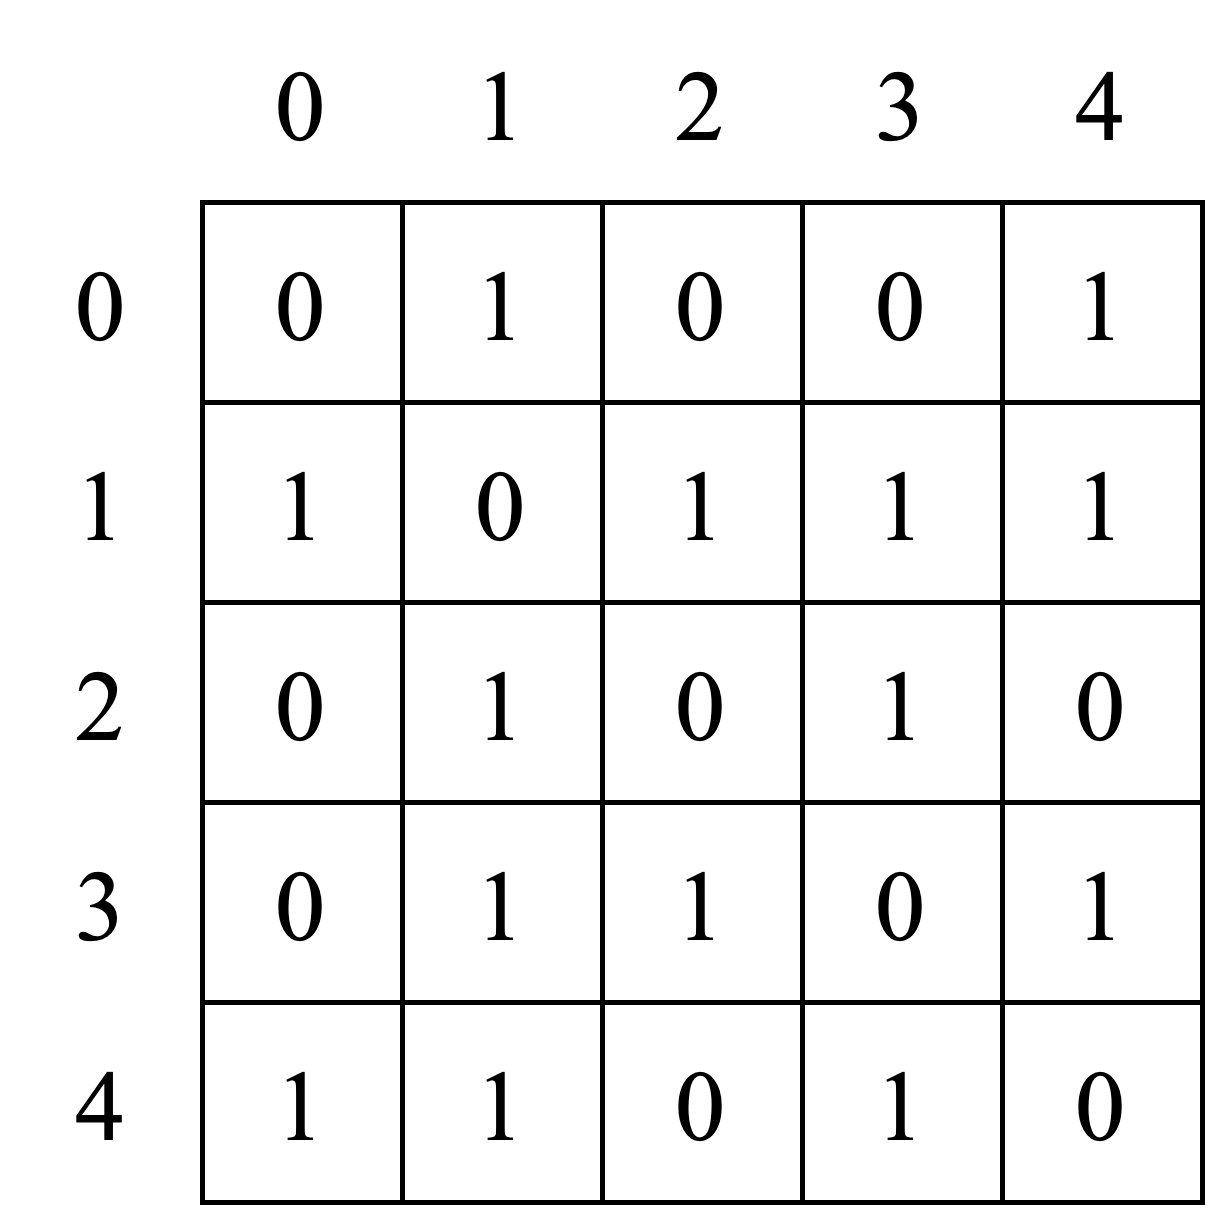
\includegraphics[width=0.4\textwidth]{adjacency_matrix}
    \caption{An adjacenecy matrix representation of a graph}
    \label{fig:adjacency_matrix}
\end{figure}

\subsubsection{Adjacency List}

\paragraph{}
Adjacency list sacrifices the cost of insertion, deletion and edge query operations in order to save space. It takes \(O(V)\)for en operation like insertion while maintaining \(O(V+E)\) cost for storing the data structure. This data structure consists of multiple lists of memory blocks which depict the edges of each vertice. The \autoref{fig:adjacency_list} is the adjacency list representation of the same graph in \autoref{fig:simple_graph}.

\begin{figure}[H]
    \centering 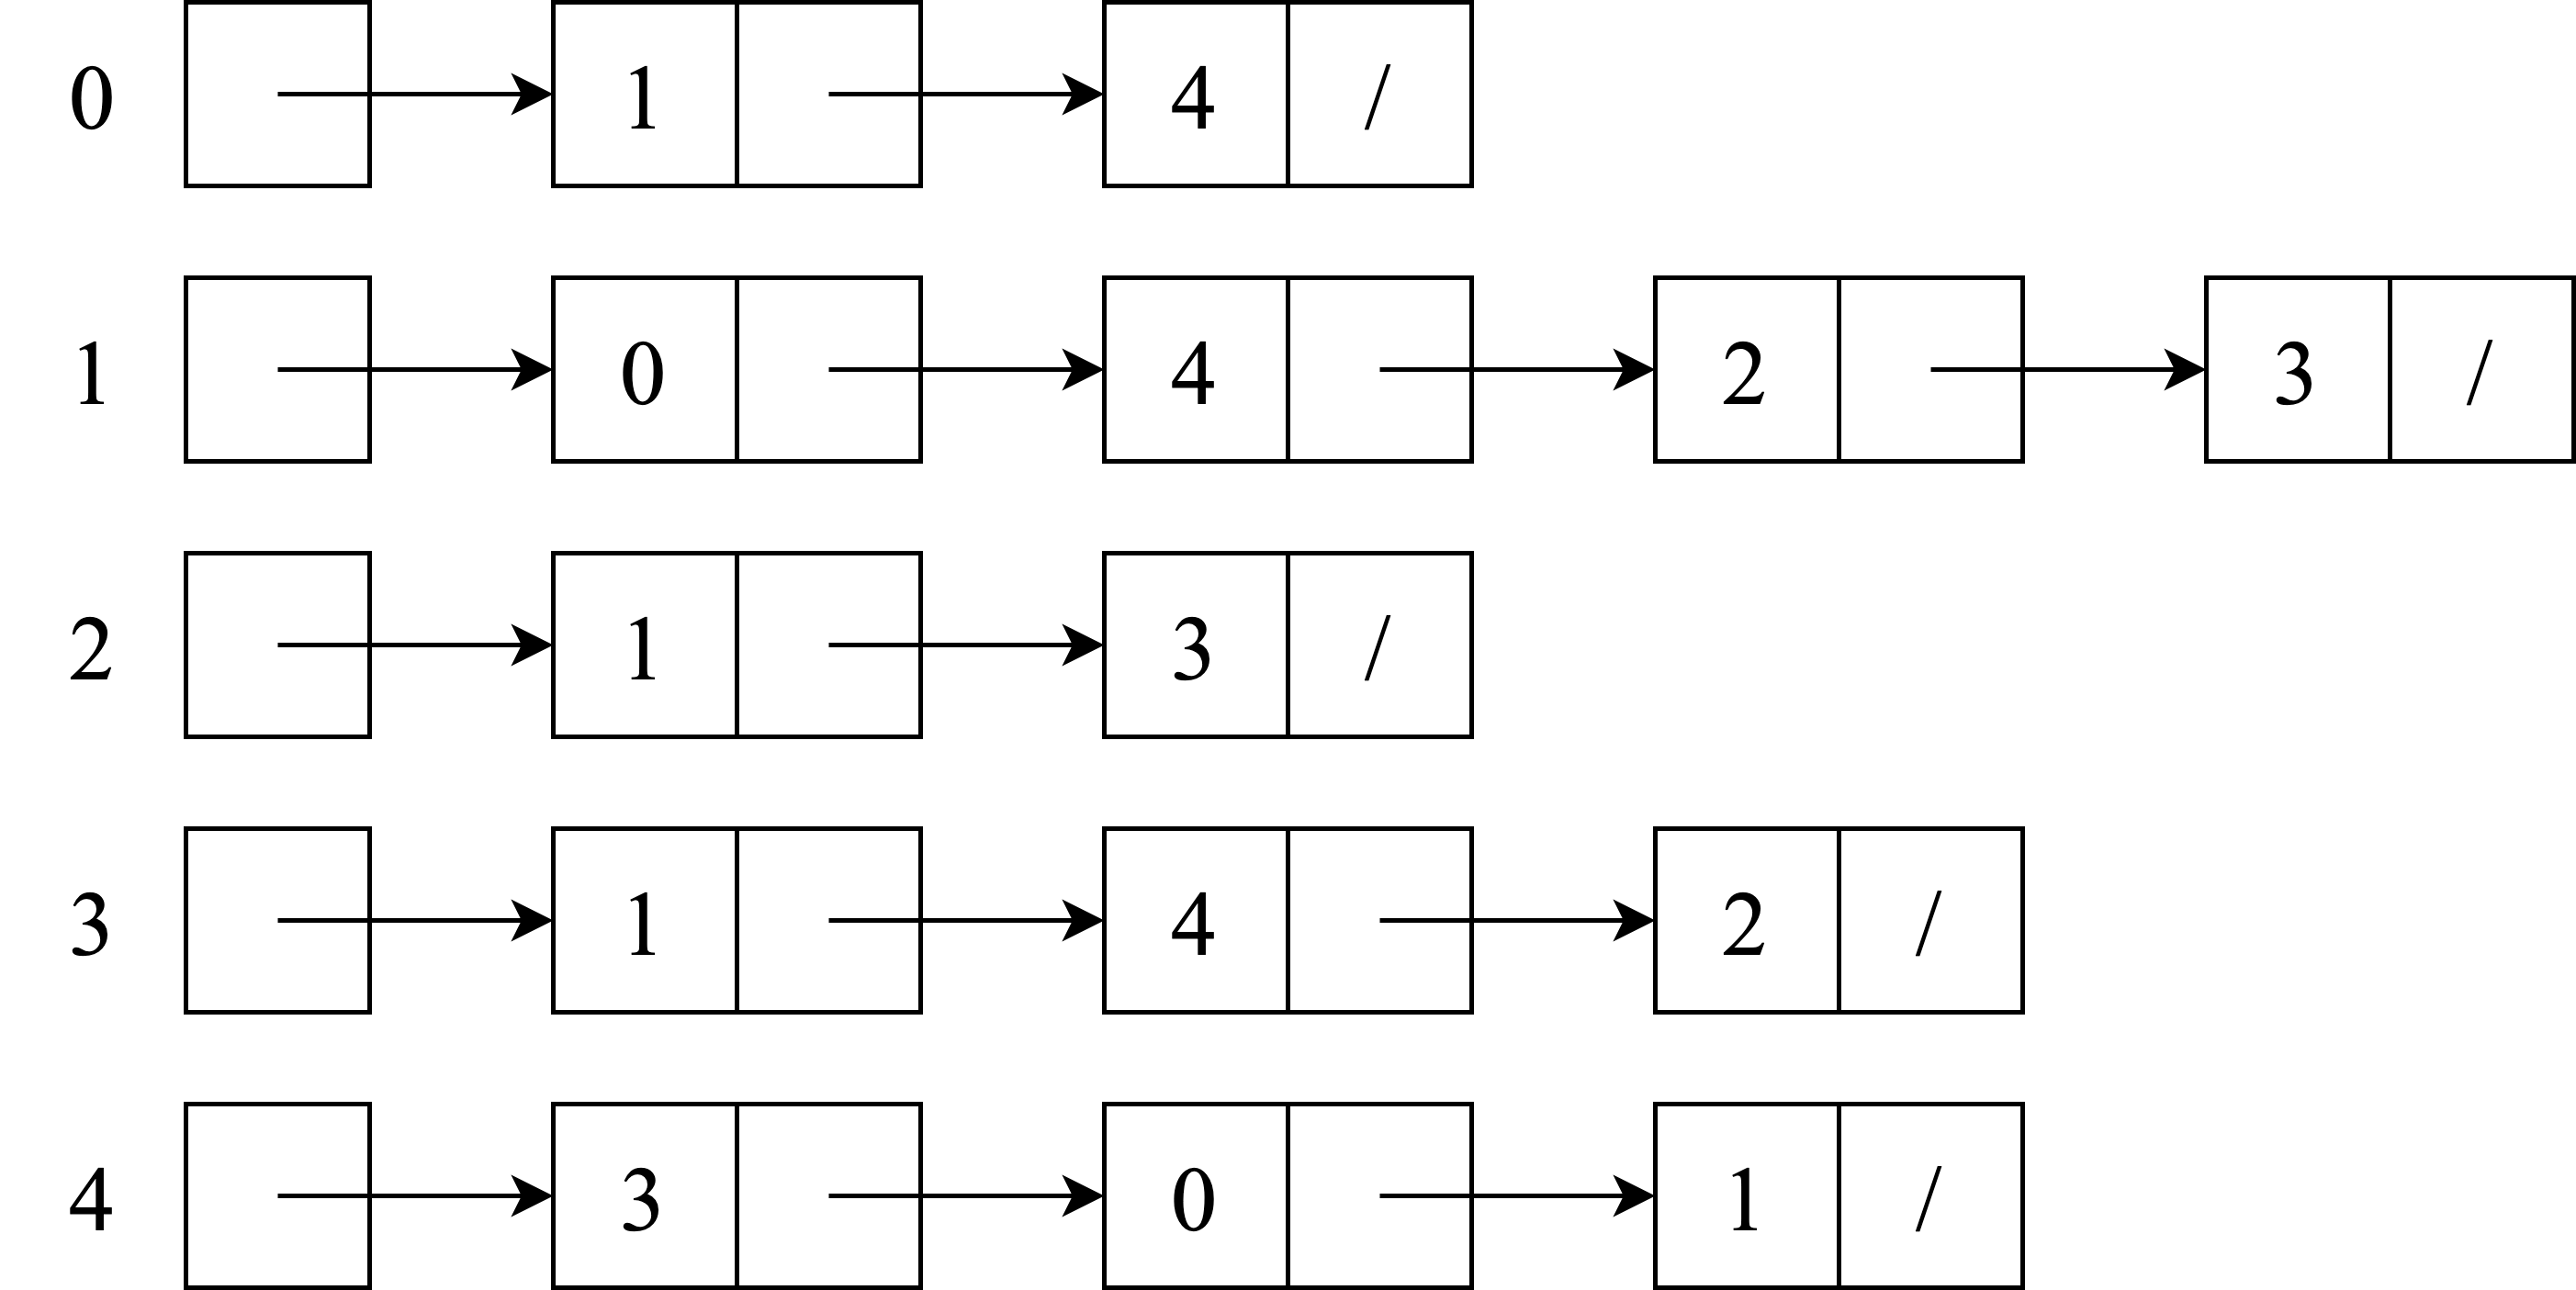
\includegraphics[width=0.85\textwidth]{adjacency_list}
    \caption{An adjacenecy list representation of a graph}
    \label{fig:adjacency_list}
\end{figure}